% CVPR 2026 camera-ready format.
% Official author kit: https://github.com/cvpr-org/author-kit
\documentclass[10pt,twocolumn,letterpaper]{article}

\usepackage{cvpr}
\usepackage{fontspec}
\usepackage{xeCJK}
\usepackage{amsmath,amssymb,mathtools}
\usepackage{graphicx}
\usepackage{booktabs}
\usepackage{array}
\usepackage{enumitem}
\usepackage{xcolor}
\usepackage{microtype}
\usepackage{balance}
\usepackage{cuted}
\usepackage{caption}

\definecolor{cvprblue}{rgb}{0.21,0.49,0.74}
\usepackage[breaklinks,colorlinks,allcolors=cvprblue]{hyperref}

\defaultfontfeatures{Ligatures=TeX}
\setmainfont{Times New Roman}
\setsansfont{Arial}
\setmonofont{Consolas}
\setCJKmainfont{Batang}
\setCJKsansfont{Malgun Gothic}
\setCJKmonofont{Malgun Gothic}

\hypersetup{
  pdftitle={Beyond FFT: Frequency vs. Variance vs. Sparsity},
  pdfauthor={Tae Joo Lee; Jang Ho Park; Yeseo Park},
  pdfsubject={Vision Transformer stability scores and high-norm artifacts},
  pdfkeywords={Vision Transformer, FFT, variance, sparsity, TASC, localization}
}

\captionsetup{font=small,labelfont=bf}
\setlist{nosep,leftmargin=1.4em}
\def\paperID{0000}
\def\confName{CVPR}
\def\confYear{2026}

\newcommand{\method}[1]{\textsc{#1}}
\newcommand{\rawscore}{\texttt{raw\_score}}
\newcommand{\votecount}{\texttt{vote\_count}}
\newcommand{\pooled}{\texttt{pooled}}

\title{Beyond FFT: Frequency vs. Variance vs. Sparsity}

\author{Tae Joo Lee\textsuperscript{*}\qquad
Jang Ho Park\textsuperscript{*}\qquad
Yeseo Park\textsuperscript{*}\\
Kyung Hee University\\
{\tt\small leetj3610@khu.ac.kr \quad pjh0846@khu.ac.kr \quad yeseo@khu.ac.kr}\\[-1pt]
{\small\textsuperscript{*}Equal contribution.}}

\begin{document}
\maketitle

\begin{abstract}
Large-scale pre-trained Vision Transformers (ViTs) commonly exhibit high-norm artifacts, where uninformative background patches show abnormally large output norms. The prior work LaSt-ViT attributes this to lazy aggregation and assumes that foreground patches have low channel-wise variance, selecting them via an FFT-based stability score. However, the ViT channel axis has no inherent ordering---permuting channels leaves the computation unchanged---whereas the FFT measures an ordering-dependent frequency structure rather than the statistical variance the premise claims. From this gap, we derive and compare three score functions on a fixed backbone: TCIG (direct neighboring-channel differences), Global Variance (direct variance), and TASC (activation spikiness via an L1/L2 ratio). On ImageNet-100, all methods reach comparable Top-1 accuracy (90--92\%), but in localization (PiB), TASC attains 65.31\% \rawscore{}---about 2.3$\times$ that of FFT (28.42\%). Notably, although both Global Variance and TASC are permutation invariant, they differ by roughly 4.2$\times$ in \votecount{} (13.57\% vs. 57.19\%), showing that permutation invariance alone is insufficient and that the artifact stems from spikes in a few channels rather than from variance itself.
\end{abstract}

\begin{strip}
\centering
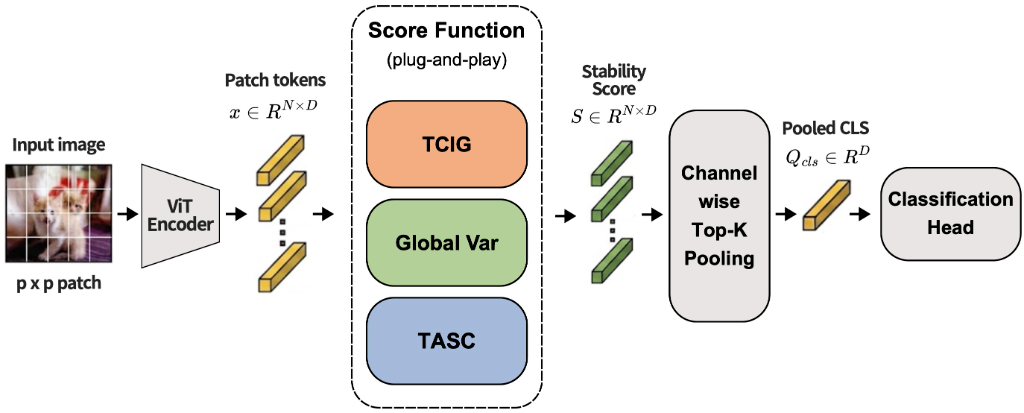
\includegraphics[width=0.94\linewidth]{figures/method_overview.png}
\captionof{figure}{Overview of the controlled comparison. The LaSt-ViT aggregation backbone is fixed while only the stability score is replaced by FFT, TCIG, Global Variance, or TASC.}
\label{fig:overview}
\end{strip}
\section{서론}

Vision Transformer (ViT) \cite{dosovitskiy2021}는 이미지 분류, 객체 탐지, 분할 등 다양한 컴퓨터 비전 과제에서 탁월한 성능을 보여왔다. 그러나 충분히 학습된 대규모 ViT 모델에서는 특정 패치 토큰의 출력 norm이 주변 토큰 대비 약 10배 이상 비정상적으로 커지는 high-norm artifact 현상이 관찰된다 \cite{darcet2024}. 이 현상은 주로 의미 정보가 희소한 배경 패치에서 발생하며, dense prediction과 객체 탐지 등 하위 과제의 성능을 저하시키는 원인으로 지목된다.

Darcet et al. \cite{darcet2024}은 high-norm artifact를 최초로 체계적으로 분석하였다. 이들은 해당 outlier 토큰이 주로 이웃 패치와의 코사인 유사도가 높은, 즉 의미 정보가 희소한 배경 패치에서 발생하며, 위치 정보나 픽셀 수준의 정보를 거의 담고 있지 않은 반면 전역적인 이미지 분류 정보는 오히려 풍부하게 인코딩하고 있음을 probing 실험을 통해 규명하였다. 이러한 관찰로부터 저자들은 모델이 정보량이 적은 배경 패치를 전역 의미 정보의 내부 저장소로 전용한다는 가설을 제시하였으며, 이를 해결하기 위해 입력 시퀀스에 별도의 학습 가능한 register token을 추가하는 방법을 제안하였다. Register 토큰을 도입하면 high-norm artifact가 사라지고, dense prediction 및 객체 탐지 성능이 향상되며, DINOv2 \cite{oquab2024}와 같은 자기지도 학습 모델에서 해석 가능한 어텐션 맵이 회복됨을 확인하였다.

그러나 Register 접근은 artifact를 흡수할 뿐 배경 패치가 high-norm을 갖게 되는 근본적인 원인을 제거하지는 않는다. 이에 대한 보다 직접적 접근으로 Shi et al. \cite{shi2026}의 LaSt-ViT가 제안되었다. 이들은 ViT가 학습 초기부터 CLS 토큰을 전경 패치보다 배경 패치와 높은 유사도를 갖도록 학습하는 lazy aggregation 패턴을 보임을 밝혔다. 이를 해결하기 위해 LaSt-ViT를 제안하며, ``전경 패치는 채널 방향 분산이 작다''는 전제 하에 FFT 기반 stability score로 변동성이 낮은 전경 패치만을 선별해 channel-wise top-$K$ pooling으로 새로운 CLS 표현을 구성한다. 이 접근은 12개 다운스트림 벤치마크에서 일관된 향상을 달성하였다.

그러나 본 논문은 LaSt-ViT의 핵심 전제와 실제 측정 수단 사이에 근본적인 간극이 존재함을 지적한다. 첫 번째 층위는 ViT 채널 축의 구조적 특성이다. ViT의 채널 축(패치 임베딩)은 학습 과정에서 결정된 basis vector들의 내적으로 구성되며, 채널 번호를 임의로 뒤섞어도 모델의 연산 결과가 완전히 동일하다. CNN과 달리 채널 간 물리적 연속성이 없으므로, 채널 인덱스를 순서 있는 1차원 신호로 취급하여 주파수 관계를 계산하는 FFT의 ordering 전제가 이론적으로 취약하다. 더욱이 ViT 학습 과정은 이러한 채널 구조를 명시적으로 강제하지 않으므로, ordering이 학습을 통해 자연스럽게 형성되는지 자체가 불분명하다.

두 번째 층위는 전제와 측정 수단의 간극이다. LaSt-ViT의 전제는 ``채널 방향 분산''에 대한 것이지만, FFT가 실질적으로 측정하는 것은 저주파 잔차 비율, 즉 ordering에 의존하는 주파수 구조이지 순수한 통계적 분산이 아니다. 채널 값이 $[1,1,1,10,10,10,10]$인 패치와 $[1,10,1,10,1,10,1]$인 패치는 통계적 분산이 동일하지만 FFT score는 전자가 훨씬 높다. 즉 FFT는 분산이 아닌 채널 ordering에 의존하는 주파수 구조를 측정한다.

이 간극에서 세 가지 자연스러운 탐색 방향이 도출된다. 각 방향은 ``FFT score가 실제로 측정하는 것은 무엇인가''라는 단일 물음에 서로 다른 각도로 접근하며, 동일한 aggregation backbone 위에서 score function만 교체하는 plug-and-play 방식으로 비교된다.

\paragraph{RQ1 -- FFT 없이 채널 ordering만 인정한 더 단순한 방법도 같은 효과를 내는가?}
FFT의 low-pass 필터가 사실상 로컬 평활화 연산에 가깝다면, 동일한 직관을 채널 ordering 전제는 유지하되 복잡한 주파수 연산 없이 이웃 채널 간 차이를 직접 측정하는 방식으로 구현할 수 있다. 만약 이 단순화가 FFT와 동등하거나 더 나은 성능을 보인다면, FFT에서 유효한 정보는 주파수 분해가 아닌 국소적 채널 유사성이며 복잡한 주파수 연산은 불필요하다는 결론이 된다.

\paragraph{RQ2 -- LaSt-ViT의 가정대로 분산을 직접 측정하면 어떻게 되는가?}
LaSt-ViT의 전제는 ``채널 방향 분산''을 명시하지만 FFT는 분산을 직접 측정하는 수단이 아니다. 따라서 ordering 전제를 완전히 폐기하고 분산을 직접 측정하는 것이 더 나은 결과를 낳는지 검증한다. RQ1과 함께 비교하면, 두 결과의 차이로부터 채널 ordering이 localization 능력에 실질적으로 기여하는지를 직접 분리해낼 수 있다.

\paragraph{RQ3 -- Artifact의 본질은 분산 전체가 아닌 소수 채널의 spike인가?}
배경 패치에서 실제로 관찰되는 현상은 채널 전반의 분산이 크다기보다, 소수의 채널에 activation이 비정상적으로 집중되는 spikiness에 더 가깝다. 이 관점에서 FFT가 효과를 보이는 이유는 주파수 원리가 아니라 spike 채널이 인접 채널과의 급격한 변화를 일으킬 때 이를 간접적으로 포착하는 부수적 효과일 수 있다. 따라서 이 spikiness를 ordering에 전혀 의존하지 않고 직접 측정하는 것이 더 근본적인 접근인지를 검증한다.

본 논문의 주요 기여는 다음과 같다. 첫째, LaSt-ViT의 FFT score가 표방하는 분산 측정과 실제 측정 수단 사이의 간극을 분석하고, 이로부터 세 가지 탐색 방향을 도출하는 분석 프레임워크를 제시한다. 둘째, 각 방향을 구체화한 세 가지 score function을 제안한다. FFT의 ordering 전제를 인정하되 복잡한 주파수 연산을 제거하고 이웃 채널 간 변화량을 직접 측정하는 TCIG (Token-Channel Independent Gating), ordering 전제를 완전히 폐기하고 채널 분산을 직접 측정하는 Global Variance, 그리고 분산이라는 개념 틀을 재해석하여 채널 activation의 spikiness를 ordering 없이 직접 감지하는 TASC (Token Activation Spike Clipping)가 그것이다. 셋째, 세 가지 대안을 동일한 환경에서 FFT와 비교하고, 각 score function이 artifact를 포착하는 메커니즘의 차이를 실험적으로 규명한다.

\section{관련 연구}

\subsection{ViT의 Artifact와 Register Token}

Darcet et al. \cite{darcet2024}은 충분히 학습된 대규모 ViT에서 전체 패치의 약 2\%에 해당하는 토큰이 주변 토큰 대비 약 10배 이상 높은 norm을 갖는 high-norm artifact 현상을 최초로 체계적으로 분석하였다. 이들은 해당 outlier 토큰이 주로 이웃 패치와의 코사인 유사도가 높은, 즉 의미 정보가 희소한 배경 패치에서 발생하며, 위치 정보나 픽셀 수준의 정보를 거의 담고 있지 않은 반면 전역적인 이미지 분류 정보는 오히려 풍부하게 인코딩하고 있음을 probing 실험을 통해 규명하였다. 이러한 관찰로부터 저자들은 모델이 정보량이 적은 배경 패치를 전역 의미 정보의 내부 저장소로 전용한다는 가설을 제시하였으며, 이를 해결하기 위해 입력 시퀀스에 별도의 학습 가능한 register token을 추가하는 방법을 제안하였다. Register 토큰을 도입하면 high-norm artifact가 사라지고, dense prediction 및 객체 탐지 성능이 향상되며, DINOv2 \cite{oquab2024}와 같은 자기지도 학습 모델에서 해석 가능한 어텐션 맵이 회복됨을 확인하였다. 그러나 이 접근은 artifact를 사후적으로 흡수하는 방식으로, 배경 패치가 high-norm을 갖게 되는 근본적인 원인을 제거하지는 않는다는 한계가 있다.

\subsection{Lazy Aggregation과 LaSt-ViT}

Shi et al. \cite{shi2026}은 register 토큰이 high-norm artifact를 제거하더라도 CLS 토큰이 배경 패치에 집중하는 근본적 편향은 해소하지 못함을 지적한다. 이들은 토큰과 각 패치 간 코사인 유사도로 정의되는 Patch Score와, 유사도가 가장 높은 패치가 전경 bounding box 안에 위치하는 비율을 측정하는 PiB 지표를 도입하여, ViT가 학습 초기부터 배경 패치를 통해 전역 의미를 우회 표현하는 lazy aggregation 패턴을 정량화하였다.

이를 해결하기 위해 LaSt-ViT는 ``전경 패치는 채널 방향 분산이 작다''는 전제 하에 FFT 기반 stability score를 도입한다. 각 패치 임베딩의 채널 축에 1D FFT를 적용하고 Gaussian low-pass 필터를 통과시킨 뒤 IFFT로 복원한 값과 원본의 비율로 stability를 정의한다. 변동성이 낮은, 즉 score가 높은 전경 패치만을 선별하여 channel-wise top-$K$ pooling으로 새로운 CLS 표현을 구성하고, 이를 분류 헤드에 전달한다. 이 접근은 기존 ViT 구조를 변경하지 않고 score function만 교체하는 plug-and-play 방식으로 설계되어 12개 다운스트림 벤치마크에서 일관된 향상을 달성하였다.

그러나 FFT는 채널 축을 순서 있는 1차원 신호의 시간 축으로 취급하여 인접 채널들 간의 주파수 관계를 계산하는 연산으로, 전제가 명시하는 통계적 분산과 동치가 아니다. 분산이 동일한 두 패치라도 채널 배열 순서가 다르면 전혀 다른 FFT score를 산출한다. 또한 표준 ViT 학습에는 이러한 채널 ordering을 명시적으로 정렬하는 메커니즘이 존재하지 않으므로, FFT가 가정하는 채널 구조가 실제로 형성되는지 자체가 불분명하다. 본 논문은 이 간극, 즉 전제와 측정 수단의 불일치를 출발점으로 삼아 분산을 직접 측정하거나 전제 자체를 재해석하는 대안적 score function을 탐색한다.

\section{제안 방법}

\subsection{전체 구조}

본 논문은 LaSt-ViT \cite{shi2026}의 channel-wise top-$K$ aggregation 구조를 backbone으로 고정하고, score function만을 교체하는 plug-and-play 방식으로 세 가지 대안을 구현한다. 입력 패치 특징과 score는
\begin{equation}
x\in\mathbb{R}^{B\times N\times D},\qquad
S\in\mathbb{R}^{B\times N\times D}
\end{equation}
이며, 채널별 top-$K$ pooling은
\begin{equation}
Q_{\mathrm{CLS}}[j]=\frac{1}{K}
\sum_{i\in\operatorname{TopK}(S[:,j])}x[i,j]
\end{equation}
로 새로운 CLS 표현을 구성한다. 이때 $K=7$로 설정한다. 손실 함수는 표준 cross-entropy만을 사용하며, score function 외의 추가적인 학습 목표는 도입하지 않는다. 네 가지 score function---FFT (baseline), TCIG, Global Variance, TASC---은 모두 동일한 aggregation backbone 위에서 score function만 교체되므로, 성능 차이를 온전히 score function 설계에 귀속시킬 수 있다.


\subsection{FFT (Shi 2026 Baseline)}

Shi et al. \cite{shi2026}의 FFT 기반 score를 그대로 재현하여 baseline으로 사용한다. 채널 축으로 1D FFT를 적용하고 Gaussian low-pass 필터 $g$를 통과시킨 후 IFFT로 복원한 값 $\hat{x}$와 원본 $x$의 비율로 stability를 정의한다.
\begin{align}
\hat{x} &= \operatorname{IFFT}(\operatorname{FFT}(x)\odot g),\\
S_{\mathrm{FFT}} &= \frac{\hat{x}}{|\hat{x}-x|+\epsilon}.
\end{align}
Score가 높다는 것은 원본 $x$와 저주파 통과 결과 $\hat{x}$의 차이가 작다는 것, 즉 해당 채널이 인접 채널들과 유사한 값을 가지며 채널 방향으로 부드럽다는 의미다. Gaussian 필터의 $\sigma$ 및 모든 hyperparameter는 Shi et al.의 공식 구현을 그대로 사용하였다. 앞서 분석하였듯이 이 score는 채널 배열 순서에 전역적으로 의존하며 통계적 분산의 올바른 측정 수단이 아니다.

\subsection{TCIG (Token-Channel Independent Gating)}

TCIG는 FFT의 ordering 전제를 그대로 인정하되, 복잡한 주파수 연산을 제거하고 이웃 채널 간 변화량을 더 직접적으로 측정하는 방법이다. FFT의 Gaussian low-pass 필터가 사실상 채널 방향의 국소 평활화 연산에 가깝다는 관찰에서 출발하여, 이를 크기 $k=7$의 1D AvgPool 슬라이딩 윈도우로 대체한다. 채널 축을 따라 윈도우를 슬라이딩하여 각 채널 위치에서 이웃 채널의 평균 $\hat{x}$를 계산하며, 가장자리 채널의 왜곡 방지를 위해 replicate padding을 적용한다.

원본과 평활화 결과의 차이를 정규화한 ratio와 stability score는
\begin{align}
r &= \frac{\bigl||x|-|\hat{x}|\bigr|}{|x|+|\hat{x}|+\epsilon},\\
S_{\mathrm{TCIG}} &= \exp(-r)
\end{align}
로 정의한다. 채널이 고를수록 $r\to0$, spike가 있을수록 $r\to1$이 된다. 따라서 ratio가 작으면 $S\approx1$로 안정적인 채널이 Top-$K$에 선택되고, ratio가 크면 score가 낮아져 spike가 있는 채널이 제외된다. TCIG는 FFT와 마찬가지로 채널 ordering에 의존하므로, 그 성능은 ViT 학습 과정에서 국소적 채널 ordering 구조가 실제로 형성되는지를 검증하는 간접 증거가 된다.

\subsection{Global Variance}

Global Variance는 ``분산을 직접 측정하면 충분하다''는 가장 단순한 가설에서 출발한다. 패치의 채널 전체에 대한 평균과 표준편차를
\begin{equation}
\mu=\frac{1}{D}\sum_{c=1}^{D}x_c,\qquad
\sigma=\sqrt{\frac{1}{D}\sum_{c=1}^{D}(x_c-\mu)^2}
\end{equation}
로 계산하고, negative z-score를
\begin{equation}
S_{\mathrm{GVar}}=-\frac{x-\mu}{\sigma+\epsilon}
\end{equation}
로 정의한다. 부호를 음수로 취하므로 평균보다 큰 양의 편차 채널일수록 낮은 score를, 평균보다 작은 채널일수록 높은 score를 받는다. 즉 이 score는 편차를 대칭적으로 다루는 순수 분산이 아니라, 양의 편차에 선택적으로 반응하는 비대칭 지표다. 이는 FFT가 양수 쪽 큰 활성(spike)을 포착하도록 설계된 방향성을 ordering 없는 변량 관점으로 옮기기 위함이다. 다만 \rawscore{}처럼 score를 채널 방향으로 합산하면 양·음 편차가 $\sum_d S\approx0$으로 패치마다 상쇄되므로, 이 방법에서 \rawscore{}는 구조적으로 불안정한 지표다. 평균과 표준편차는 집합 연산으로 계산되므로 채널 순서에 permutation invariant하다.

\subsection{TASC (Token Activation Spike Clipping)}

TASC는 전제를 ``채널 분산이 작다''가 아닌 ``채널 activation이 고르다''로 재해석하고, 이를 채널 ordering 없이 직접 감지한다. 전경 패치는 채널 전반에 activation이 고르게 분포하는 반면, 배경 패치는 일부 채널만 극단적으로 큰 값을 가지고 나머지는 매우 작은 값을 갖는 불균일한 분포를 보인다. Activation 분포의 균일도를 측정하기 위해 L1/L2 norm ratio를 활용한다.
\begin{align}
L_1 &= \frac{1}{D}\sum_{c=1}^{D}|x_c|,\qquad
L_2 = \sqrt{\frac{1}{D}\sum_{c=1}^{D}x_c^2},\\
\alpha &= \frac{L_1}{L_2},\qquad \alpha\in[1/\sqrt{D},1].
\end{align}
모든 채널의 절댓값이 동일한 완전 균일 분포에서는 $\alpha=1$이며, 소수의 채널에 activation이 집중될수록 $\alpha$는 하한인 $1/\sqrt{D}$ 방향에 가까워진다. 클리핑 계산은 $\alpha$로 동적으로 결정된 임계값을 사용한다.
\begin{align}
\tau &= L_1\cdot\alpha,\\
\hat{x} &= \operatorname{sign}(x)\cdot\min(|x|,\tau),\\
S_{\mathrm{TASC}} &= \frac{|\hat{x}|^2}{|x|+\epsilon}.
\end{align}
전경 패치는 activation이 고르게 분포하므로 $\alpha\simeq1$이 되어 임계값이 충분히 크고 대부분의 채널이 클리핑되지 않는다. 반면 배경 패치는 $\alpha\ll1$이 되어 임계값이 낮아지고 spike 채널에서 클리핑이 발생한다. TASC는 L1, L2, $\alpha$가 모두 집합 연산으로 계산되므로 채널 순서에 완전히 독립적이며, 분산이 아닌 activation의 절대적 극단성을 측정한다.

\section{실험 및 결과}

\subsection{데이터셋 및 구현 세부사항}

\paragraph{데이터셋.}
실험에는 ImageNet-1k \cite{russakovsky2015}에서 100개 클래스를 균등 선별한 ImageNet-100을 사용한다. Train set은 약 130k 이미지, Validation set은 5k 이미지로 구성된다. 전체 1k 클래스 대비 규모를 줄여 실험 효율을 확보하되, 다양한 시각적 범주를 포함하도록 구성하여 일반화 가능한 비교가 이루어지도록 하였다.

\paragraph{Backbone 및 학습 설정.}
Backbone은 ViT-S/16 ($D=384$, depth$=12$, heads$=6$)을 사용한다. ImageNet-1k pretrained 가중치로 초기화한 뒤 fine-tuning하는 것을 기본 설정으로 하며, score function은 pretrained encoder 위에 plug-and-play 방식으로 장착된다. 분류 head는 ImageNet-1K 사전학습 가중치에서 대상 100개 클래스에 해당하는 행을 슬라이싱하여 초기화하였으며, score function과 aggregator는 랜덤 초기화하였다. Optimizer는 AdamW, learning rate는 $5\times10^{-4}$를 사용한다. 총 100 epoch, batch size 256으로 학습하며, data augmentation은 DeiT-III \cite{touvron2022} 레시피를 따라 Mixup, CutMix, RandAugment를 적용한다. Top-$K$는 기본 실험에서 $K=7$로 설정한다. 학습에는 NVIDIA A6000과 RTX 2080 GPU를 사용하였다.

\subsection{평가 지표}

분류 성능은 Top-1 Accuracy로 평가한다. 그러나 본 논문의 핵심 관심사는 각 score function이 전경 패치를 얼마나 정확하게 식별하는가이므로, localization 성능을 주된 평가 기준으로 삼는다. Localization 평가에는 LaSt-ViT \cite{shi2026}가 도입한 Point-in-Box (PiB) 지표를 사용한다. PiB는 stability score 기준으로 가장 높은 score를 받은 패치가 Ground Truth Bounding Box 내에 위치하는지를 측정하고, 이를 validation set 전체에 대해 평균한 값이다.

PiB는 세 가지 변형으로 측정한다. \rawscore{}는 각 토큰의 stability score를 채널 방향으로 합산하여 패치를 직접 랭킹하는 방식이며 본 논문의 주된 비교 기준이다. \votecount{}는 채널별 Top-$K$ 투표를 집계하는 방식으로 LaSt-ViT가 직접 정의한 metric이다. \pooled{}는 집계된 CLS와의 코사인 유사도를 기반으로 하며, 선택된 패치로 만든 pooled CLS와의 재비교이므로 순환 가능성이 있어 보조 지표로만 참고한다.

\subsection{주요 결과}

\begin{table}[t]
\centering
\caption{ImageNet-100, pretrained fine-tuning, $K=7$.}
\label{tab:main}
\resizebox{\columnwidth}{!}{%
\begin{tabular}{lrrrr}
\toprule
Method & \rawscore{} & \votecount{} & \pooled{} & Top-1 \\
\midrule
FFT (baseline) & 28.42 & 22.74 & 38.17 & 92.30 \\
TCIG & 29.47 & 22.04 & 18.45 & \textbf{92.34} \\
Global Var & 9.40 & 13.57 & \textbf{67.29} & \textbf{92.34} \\
TASC & \textbf{65.31} & \textbf{57.19} & 62.53 & 92.16 \\
Vanilla$^{*}$ & -- & -- & 48.49 & 90.32 \\
\bottomrule
\end{tabular}}
\vspace{0.2em}
\caption*{$^{*}$Vanilla는 선택적 집계를 적용하지 않아 분류 경로가 구조적으로 다르며, 집계 미적용 시의 참고 상한으로만 사용한다.}
\end{table}

Top-1 정확도는 모든 방법이 90--92\% 수준으로 유사하여, score function 간 변별력은 localization 지표에서 나타난다.

\paragraph{RQ1 (TCIG).}
TCIG는 \rawscore{} 29.47\%, \pooled{} 18.45\%를 기록하였다. 주지표인 \rawscore{}에서 TCIG(29.47\%)와 FFT(28.42\%)는 거의 동등한 수준으로, TCIG는 FFT에 대해 안정적인 우위를 보이지 않으며 \pooled{}에서는 오히려 크게 뒤처진다. FFT의 ordering 전제를 인정하면서 연산만 단순화한 TCIG가 FFT를 일관되게 능가하지 못한다는 사실은, 채널 순서가 없는 ViT에서 이웃 채널 간 차이를 빼는 연산이 전경과 배경의 에너지를 무차별적으로 건드려 신호를 효과적으로 살리지 못함을 시사한다.

\paragraph{RQ2 (Global Variance).}
Global Variance는 \pooled{} 67.29\%로 FFT(38.17\%)를 크게 상회하였으나, \rawscore{}는 9.40\%로 FFT(28.42\%)보다 현저히 낮다. 이 낮은 \rawscore{}는 score에 전경 신호가 없어서가 아니라, 부호 있는 z-score를 채널 방향으로 합산할 때 양·음 편차가 상쇄되어 패치마다 $\sum_d S\approx0$으로 무너지는 구조적 degeneracy에서 비롯된다. 즉 \rawscore{}는 이 방법에서 신뢰 지표가 되지 못하며, \pooled{}의 개선은 pooled CLS와의 상호작용에서 비롯된 결과일 가능성이 크다. 신뢰 가능한 \votecount{} 기준으로는 FFT에 미치지 못해(13.57\% vs. 22.74\%), 분산이 곧 artifact의 본질은 아니라는 신호다.

\paragraph{RQ3 (TASC).}
TASC는 \rawscore{} 65.31\%, \votecount{} 57.19\%, \pooled{} 62.53\%를 기록하였으며, \rawscore{}와 \votecount{}에서 1위를 차지하였다. \rawscore{} 기준으로 FFT(28.42\%)의 약 2.3배에 달한다. Global Variance와 TASC 모두 permutation invariant임에도 \votecount{}에서 13.57\% vs. 57.19\%로 약 4.2배 차이가 발생한다는 사실은, 순열 불변성 자체가 고성능의 충분조건이 아님을 보여준다. Artifact의 본질이 ``분산이 크다''가 아니라 ``소수 채널에 에너지가 쏠린 spike''임을 강하게 시사하며, FFT의 효과 역시 주파수 원리가 아닌 spike를 우연히 깎은 부수 효과에 가깝다는 해석을 지지한다.

\begin{figure*}[t]
\centering
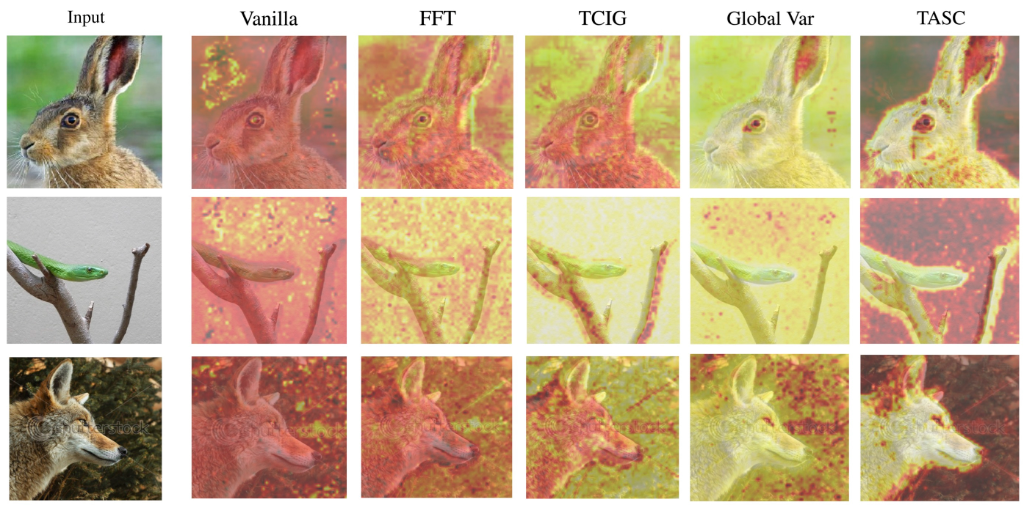
\includegraphics[width=0.96\textwidth]{figures/feature_norm_overlay.png}
\caption{각 score function의 feature norm을 입력 이미지에 overlay한 시각화. 밝은색일수록 norm이 높음을 의미한다.}
\label{fig:norm}
\end{figure*}

그림 \ref{fig:norm}은 각 방법의 feature norm 분포를 히트맵으로 시각화한 것이다. Vanilla와 FFT는 전경과 배경의 norm 분포가 뚜렷하게 구분되지 않으며, 배경 영역에도 높은 norm이 산발적으로 나타난다. TCIG는 채널 ordering 노이즈로 인해 불규칙한 패턴을 보인다. Global Variance는 전경-배경 대비가 완만하게 형성되나 경계가 불명확하다. 반면 TASC는 전경 객체와 배경의 norm 분포를 잘 구분한다.

\begin{figure*}[t]
\centering
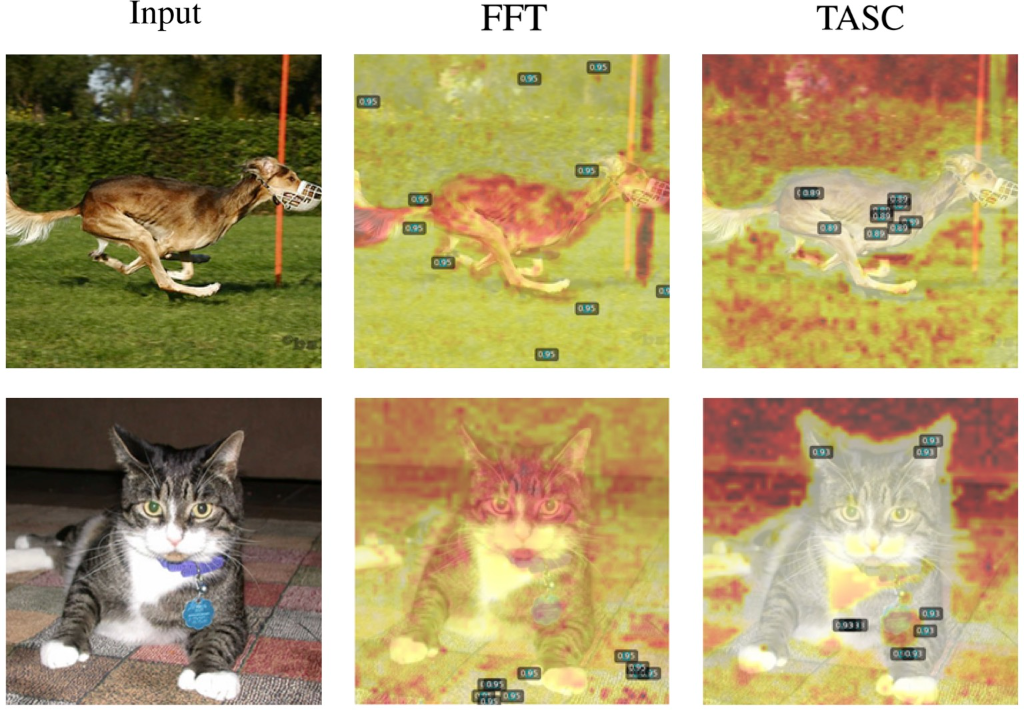
\includegraphics[width=0.86\textwidth]{figures/topk_fft_vs_tasc.png}
\caption{FFT와 TASC의 Top-$K$ 패치 선택 결과 시각화. 각 패치에 표시된 수치는 해당 패치의 score이며, 밝은 영역일수록 높은 score를 나타낸다.}
\label{fig:topk}
\end{figure*}

그림 \ref{fig:topk}는 각 방법이 실제로 선택한 Top-$K$ 패치의 위치를 FFT와 TASC 간에 직접 비교한 것이다. FFT는 전경 객체 위에도 일부 패치를 선택하지만, 배경 영역의 패치가 혼재되어 선택의 일관성이 낮다. 반면 TASC는 선택된 패치들이 전경 객체의 윤곽에 집중적으로 분포하며, 배경 영역의 패치가 효과적으로 배제됨을 확인할 수 있다. 이는 수치 결과에서 나타난 \rawscore{} 차이가 실제 패치 선택의 질적 차이에서 비롯됨을 직관적으로 보여준다.

\subsection{추가 분석}

\subsubsection{$K$값에 따른 성능 변화}

LaSt-ViT \cite{shi2026}는 $K=98$을 sweet spot으로 주장하며, 이는 FFT의 랭킹 노이즈를 평균으로 덮으려는 시도이고 $K=98$에서 배경 50\% 오염이 강제된다고 서술한다. 우리는 이에 두 가지 정정을 제시한다. 첫째, $K$는 전역 예산이 아닌 채널별 Top-$K$로, 채널마다 독립적으로 $K$개 패치를 선택하는 구조이므로 ``$K=98\to$ 배경 50\% 오염'' 산술은 성립하지 않는다. 둘째, LaSt-ViT의 $K=98$ peak는 분류 정확도 기준이며 localization(PiB)에 관한 진술이 아니다. 우리의 관점에서 $K$는 ``오염의 산술''이 아닌 ``정밀도(PiB)가 $K$에 어떻게 반응하는가''로 재해석되어야 한다.

\begin{table}[t]
\centering
\caption{ImageNet-100, pretrained fine-tuning, $K=98$.}
\label{tab:k98}
\resizebox{\columnwidth}{!}{%
\begin{tabular}{lrrrr}
\toprule
Method & \rawscore{} & \votecount{} & \pooled{} & Top-1 \\
\midrule
FFT (baseline) & 26.33 & 43.97 & 20.76 & 92.08 \\
TCIG & 18.79 & 22.85 & 21.11 & 92.28 \\
Global Var & 12.99 & 23.78 & 25.99 & \textbf{92.36} \\
TASC & \textbf{36.43} & \textbf{48.49} & \textbf{27.96} & 91.94 \\
Vanilla$^{*}$ & -- & -- & 48.49 & 90.32 \\
\bottomrule
\end{tabular}}
\end{table}

$K=98$로 넓히자 TASC \pooled{}가 $K=7$ 실험의 62.53\%에서 27.96\%로 크게 하락하였으며, FFT도 20.76\%로 낮아졌다. 넓은 $K$에서는 평균에 섞이는 패치 수가 많아져 \pooled{} 경로의 변별력 자체가 떨어지는 것으로, 이는 모듈의 결함이 아닌 집계 방식의 구조적 특성이다. 그러나 \rawscore{}(36.43\% vs. 26.33\%), \votecount{}(48.49\% vs. 43.97\%) 모두 TASC가 FFT를 상회하여, $K$가 커져 \pooled{}가 무뎌진 환경에서도 score 자체의 품질은 유지된다. FFT는 $K$를 넓혀도 PiB가 낮은 수준에 머물러 랭킹 품질 자체의 문제임이 드러나며, TASC는 예리한 $K=7$에서 큰 도약을 보여 얼마나 키우느냐가 아닌 score 품질이 핵심임을 시사한다.

\subsubsection{분산 측정 방식의 영향}

Global Variance는 채널 전체를 하나의 분포로 보는데, 채널마다 값의 크기와 분포가 달라 전체 분산을 그냥 구하는 것이 적절한지에 대한 의문이 제기될 수 있다. 채널 전체를 단일 분포로 보는 대신 크기 $w$의 window 내에서만 국소적으로 정규화하면 이 문제를 완화할 수 있는지 검증하기 위해, non-overlapping window로 채널을 분할하여 window 내에서만 분산을 측정하는 Local Window Variance ($w=8$)를 비교한다. Local Window Variance는 window 내에서만 채널 순서에 의존하며, window 경계를 넘는 채널 간에는 ordering 가정을 두지 않는다.

\begin{table}[t]
\centering
\caption{Global Variance와 Local Variance 비교.}
\label{tab:variance}
\resizebox{\columnwidth}{!}{%
\begin{tabular}{lrrrr}
\toprule
Method & \rawscore{} & \votecount{} & \pooled{} & Top-1 \\
\midrule
FFT (baseline) & 28.42 & 22.74 & 38.17 & 92.30 \\
Global Var & 9.40 & 13.57 & 67.29 & 92.34 \\
Local Var ($w=8$) & 24.01 & 17.63 & 27.61 & 92.18 \\
\bottomrule
\end{tabular}}
\end{table}

Local Variance가 Global Variance보다 \rawscore{}는 높지만(24.01\% vs. 9.40\%) \pooled{}는 오히려 낮다(27.61\% vs. 67.29\%). 국소 정규화가 \rawscore{} 기준 점수 품질은 일부 회복시키나 \pooled{} 경로에서는 Global Variance에 크게 못 미친다. 두 방법 모두 \votecount{} 기준으로 FFT(22.74\%)를 넘지 못하였으며(Global Variance 13.57\%, Local Variance 17.63\%), 이는 분산을 어떻게 정규화하느냐의 문제가 아니라 분산 자체가 artifact를 포착하는 올바른 척도가 아님을 보여준다.

\subsubsection{채널 순열 불변성 검증}

\begin{table}[t]
\centering
\caption{채널 순열 불변성 실험.}
\label{tab:perm}
\resizebox{\columnwidth}{!}{%
\begin{tabular}{lrrrc}
\toprule
Method & Identity & Permuted (mean$\pm$std) & Drop & 순서 의존 \\
\midrule
TASC & 0.9216 & 0.9216$\pm$0.0000 & $+0.0000$ & X \\
Global Var & 0.9236 & 0.9236$\pm$0.0000 & $+0.0000$ & X \\
TCIG & 0.9234 & 0.9222$\pm$0.0009 & $+0.0012$ & O \\
FFT & 0.9230 & 0.9220$\pm$0.0005 & $+0.0010$ & O \\
\bottomrule
\end{tabular}}
\end{table}

TASC와 Global Variance는 5개 seed 전부 Drop이 0.0000으로, 채널을 어떻게 섞어도 결과가 비트 단위로 동일하다. FFT와 TCIG는 순서를 섞으면 수치 변화가 발생하여 채널 ordering에 의존함이 확인된다. 표 \ref{tab:perm}의 Drop은 Identity 대비 순열 후 Top-1의 하락폭(Identity $-$ Permuted 평균)으로, 값이 양수일수록 순열에 의해 성능이 떨어졌음을 의미한다. FFT의 하락은 0.10\%p, TCIG는 0.12\%p에 불과하여, 이는 Top-1이 localization에 둔감한 지표이기 때문이며 ``FFT가 무너진다''는 해석은 적절하지 않다. 보다 중요한 관찰은 Global Variance와 TASC의 비교다. 두 방법 모두 순열 불변임에도 \votecount{}에서 13.57\% vs. 57.19\%로 약 4.2배 차이가 발생한다는 사실은, 순열 불변성 자체가 고성능의 충분조건이 아님을 보여준다.

\section{분석}

\subsection{주장 범위의 한정}

본 연구는 ``TASC가 ViT의 high-norm artifact를 근본적으로 제거하거나 ViT 자체를 고친다''고 주장하지 않는다. 본 연구가 다루는 질문은 LaSt-ViT가 제시한 channel-wise top-$K$ 선택적 집계 프레임워크를 고정한 조건 하에서, 어떤 stability score가 전경 패치를 가장 정확하게 식별하는가이다. 즉 본 연구의 기여는 새로운 아키텍처의 제안이 아니라, 동일한 집계 backbone 위에서 score function만을 교체하며 그 설계 원리를 통제된 환경에서 비교·규명하는 데 있다.

이러한 범위 한정은 기준선 설정에도 그대로 반영된다. 본 연구의 기준선은 Vanilla가 아니라 LaSt-ViT의 FFT score이다. Vanilla는 선택적 집계를 적용하지 않아 분류 경로가 구조적으로 달라, 동일한 backbone 위에서 score function의 우열을 비교한다는 본 연구의 목적과 부합하지 않는다. 따라서 Vanilla는 직접 비교 대상이 아니라 집계 미적용 시의 참고 상한으로만 각주적으로 다룬다. 모든 score function의 우열은 동일 backbone, 동일 $K$, 동일 학습 조건 하에서 FFT score와의 상대 비교로 판단된다.

\subsection{지표 선택의 정당성}

본 연구는 \rawscore{}를 주지표로 삼는다. \rawscore{}는 각 토큰의 stability score를 채널 방향으로 합산하여 패치를 직접 랭킹하는 방식으로, 추가적인 학습이나 별도의 표현 학습 없이 모듈이 산출한 점수 그 자체만으로 전경 식별 능력을 평가한다. 따라서 각 score function의 전제가 실제 전경 분포에 얼마나 부합하는지를 가장 직접적으로 검증할 수 있다.

또한 단일 지표에만 의존하면 특정 지표에 유리한 결과만 선별적으로 보고한다는 의혹을 피하기 어렵다. 이를 차단하기 위해 \rawscore{}와 함께 \votecount{}와 \pooled{}를 항상 병기한다. \votecount{}는 채널별 top-$K$ 투표를 집계하는 방식으로 LaSt-ViT가 직접 정의한 지표이며, \pooled{}는 집계된 CLS와의 코사인 유사도에 기반한다. 단, \pooled{}는 선택된 패치로 구성한 pooled CLS와의 재비교라는 순환 가능성을 내포하므로 보조 지표로만 참고한다.

\subsection{세 가설의 종합 해석: Frequency vs. Variance vs. Sparsity}

세 가지 대안은 각각 artifact의 본질에 대한 서로 다른 가설을 대표한다. FFT는 채널 ordering에 의존하는 주파수 구조(Frequency)를, TCIG는 그 주파수 연산을 이웃 채널 차이로 단순화한 변형을, Global Variance와 Local Variance는 채널 분산(Variance)을, TASC는 소수 채널의 activation 집중(Sparsity)을 측정한다.

실험 결과는 일관된 서열을 보인다. 분산 계열(Global/Local Variance)은 ordering을 폐기한 방향성은 옳았으나 \votecount{} 기준 FFT(22.74\%)를 넘지 못하여(각각 13.57\%, 17.63\%), 분산이 곧 artifact의 본질이 아님을 드러낸다. Ordering을 단순화한 TCIG 역시 FFT를 일관되게 능가하지 못한다. 반면 Sparsity를 직접 측정하는 TASC는 주지표인 \rawscore{}(65.31\% vs. FFT 28.42\%)와 \votecount{}(57.19\% vs. 22.74\%)에서 FFT를 압도하며, 보조 지표인 \pooled{}에서도 FFT를 크게 상회한다. 즉 동일 backbone, 동일 $K$, 파라미터 프리 조건에서 Sparsity가 Frequency를 주지표 전반에 걸쳐 일관되게 능가한다.

특히 Global Variance와 TASC는 모두 채널 순서에 완전히 독립적인 permutation invariant 방법임에도, \votecount{}에서 13.57\% 대 57.19\%로 약 4.2배의 차이를 보인다. 이는 순열 불변성 자체가 고성능의 충분조건이 아님을 명확히 보여준다. 또한 ordering에 의존하는 FFT와 TCIG가 Global Variance보다 높은 \votecount{}를 기록한다는 사실은, ordering 의존성의 유무보다 무엇을 측정하는가가 더 결정적임을 시사한다. 결국 TASC의 우위는 순열 불변성에서 비롯되는 것이 아니라, L1/L2 ratio를 통해 activation의 spikiness를 직접 포착한다는 측정 대상의 선택 자체에서 비롯된다. 이는 FFT가 보였던 효과 역시 주파수 원리에 기인한 것이 아니라, spike 채널이 인접 채널과 급격한 변화를 일으킬 때 이를 간접적으로 깎아낸 부수 효과에 가깝다는 해석을 뒷받침한다.

\section{결론 및 한계}

\subsection{결론}

본 연구는 LaSt-ViT의 FFT 기반 stability score가 표방하는 ``채널 방향 분산''이라는 전제와, FFT가 실제로 측정하는 ordering 의존적 주파수 구조 사이의 간극을 출발점으로 삼았다. 이 간극에서 세 가지 탐색 방향---ordering을 단순화한 TCIG, 분산을 직접 측정하는 Global Variance, spikiness를 직접 감지하는 TASC---을 도출하고, 동일한 channel-wise top-$K$ 집계 backbone 위에서 score function만을 교체하는 통제된 비교를 수행하였다. 그 결과 high-norm artifact의 본질은 채널 전반의 분산이 크다는 데 있는 것이 아니라 소수 채널에 activation이 집중되는 spike에 있으며, FFT의 효과는 주파수 원리가 아닌 이 spike를 우연히 억제한 부수 효과에 가깝다는 결론에 도달하였다. Activation의 spikiness를 직접 측정하는 TASC는 주지표 전반에서 FFT를 일관되게 능가하였고, 별도의 auxiliary loss나 추가 learnable parameter 없이 동작하며, FFT/IFFT를 요구하지 않는 L1/L2 ratio 기반 score이므로 기존 FFT 기반 LaSt-ViT보다 더 적은 연산 부담으로 동일한 선택적 집계 프레임워크에 결합될 수 있다.

\subsection{한계 및 향후 연구}

본 연구의 결론은 몇 가지 조건 하에서 도출되었다. 첫째, 모든 실험은 ImageNet-100이라는 단일 데이터셋에서 수행되었다. 전체 ImageNet-1k나 도메인이 상이한 데이터셋에서 동일한 서열이 유지되는지는 추가 검증이 필요하다. 둘째, backbone은 ViT-S/16 단일 구성에 한정되었으며, 더 큰 규모의 ViT나 다른 패치 크기에서 spike 현상의 강도와 score function의 상대적 우열이 달라질 가능성이 있다. 셋째, 본 연구는 classification fine-tuning 환경에서의 localization(PiB)을 주된 평가 기준으로 삼았으므로, 결론은 선택적 집계 프레임워크 내 stability score 비교라는 범위에 한정되며 ViT 표현 자체의 개선을 보장하지는 않는다. 넷째, 본 연구의 주요 실험 결과(표 \ref{tab:main})는 모두 단일 시드 기반으로 측정되었으며, 다중 시드에 걸친 분산 및 통계적 유의성 검증은 향후 과제로 남는다.

향후 연구로는 spikiness 기반 측정이 DINOv2 \cite{oquab2024}와 같은 자기지도 학습 모델이나 객체 탐지·분할 등 dense prediction 과제로 확장될 때에도 일관된 이점을 제공하는지 검증할 필요가 있다. 또한 artifact의 본질이 소수 채널의 spike라는 본 연구의 관찰을 학습 단계에서 직접 활용하여, 사후 선택이 아니라 학습 과정에서 spike 형성 자체를 억제하는 방향은 의미 있는 후속 과제가 될 것이다.

\balance
\begin{thebibliography}{9}
\bibitem{dosovitskiy2021}
A. Dosovitskiy et al., ``An image is worth 16$\times$16 words: Transformers for image recognition at scale,'' in \emph{Proc. Int. Conf. Learn. Represent. (ICLR)}, 2021.

\bibitem{darcet2024}
T. Darcet, M. Oquab, J. Mairal, and P. Bojanowski, ``Vision transformers need registers,'' in \emph{Proc. Int. Conf. Learn. Represent. (ICLR)}, 2024.

\bibitem{oquab2024}
M. Oquab et al., ``DINOv2: Learning robust visual features without supervision,'' \emph{Trans. Mach. Learn. Res. (TMLR)}, 2024.

\bibitem{shi2026}
C. Shi, Y. Yu, and S. Yang, ``Vision transformers need more than registers,'' in \emph{Proc. IEEE/CVF Conf. Comput. Vis. Pattern Recognit. (CVPR)}, 2026.

\bibitem{russakovsky2015}
O. Russakovsky et al., ``ImageNet large scale visual recognition challenge,'' \emph{Int. J. Comput. Vis. (IJCV)}, vol. 115, no. 3, pp. 211--252, 2015.

\bibitem{touvron2022}
H. Touvron, M. Cord, and H. J\'egou, ``DeiT III: Revenge of the ViT,'' in \emph{Proc. Eur. Conf. Comput. Vis. (ECCV)}, 2022, pp. 516--533.
\end{thebibliography}

\end{document}
